\documentclass{article}


% ready for submission
\usepackage[final]{hlt_project_template}
\usepackage{natbib}
\usepackage{float}
\usepackage{graphicx}
\bibliographystyle{plainnat}



\usepackage[utf8]{inputenc} % allow utf-8 input
\usepackage[T1]{fontenc}    % use 8-bit T1 fonts
\usepackage{hyperref}       % hyperlinks
\usepackage{url}            % simple URL typesetting
\usepackage{booktabs}       % professional-quality tables
\usepackage{amsfonts}       % blackboard math symbols
\usepackage{nicefrac}       % compact symbols for 1/2, etc.
\usepackage{microtype}      % microtypography
\usepackage{xcolor}         % colors
\usepackage{amsmath}
\usepackage{multirow}
\usepackage{siunitx}    % for \SI and \num macros (percentages, large numbers)
\usepackage{tikz}
\usetikzlibrary{positioning}


\title{Trip Advisor Reviews Sentiment Analysis using RNN and Transformers} 


\author{%
  Salvatore Mastrangelo\\
  \texttt{s.mastrangelo4@studenti.unipi.it}
}


\begin{document}

\maketitle


\begin{abstract}
This study investigates document-level sentiment classification of hotel reviews 
by contrasting a lightweight Long Short-Term Memory Recurrent Neural Network (LSTM-RNN) 
with a pretrained Transformer (RoBERTa-base) fine-tuned through Low-Rank Adaptation (LoRA). 
The analysis is conducted on 18'273 English hotel reviews trimmed to 256 tokens and 
split 72.3 / 12.7 / 15 \% for training, validation and testing, respectively, in a strongly 
imbalanced five-star rating distribution.

The LSTM comprises an embedding layer, a single LSTM layer with mean-pooled hidden states, 
and a soft-max classifier, achieving convergence below 240 s on a consumer GPU. 
A RoBERTa based model was fine-tuned with FP16 precision and a LoRA adapter, thet reduced 
trainable parameters to 1.9 \% of the backbone, enabling single-GPU training.

On the native dataset, RoBERTa outperformed the LSTM with 67 \% accuracy / weighted 
F1 = 0.67 in the five-class task and 88 \% / 0.88 in the ternary task, compared with 58 \% / 0.58 and 84 \% / 0.83 for the LSTM, respectively. 
Transformer models shows great capability in classifying minority ratings (1–3 stars). 

These findings underscore three insights: (i) pre-trained attention models confer 
a clear advantage on imbalanced, ambiguous opinion data; (ii) conventional RNNs remain 
competitive under balanced conditions and deliver rapid training; (iii) LoRA enables 
cost-effective fine-tuning of large encoders. The work thus provides a reproducible 
benchmark and practical guidelines for choosing architectures under resource and 
data-distribution constraints.

% This report presents a comprehensive analysis of sentiment classification on Trip Advisor reviews using 
% Recurrent Neural Networks (RNNs) and Transformers. The study explores the effectiveness of these models 
% in understanding and predicting sentiment from textual data. A detailed methodology, experimental setup, 
% and results are provided, highlighting the strengths and weaknesses of each approach. In particular,
% given a rather small dataset of Trip Advisor reviews, the aim is to classify the sentiment of each review into both
% stars classes (1 to 5 stars) and ternary classes (positive, negative, neutral). RNN models are implemented
% using Long Short-Term Memory (LSTM), while Transformers are implemented using the BERT architecture, in
% particular the RoBERTa model. The results show that while Transformers require much less epochs to 
% converge, RNNs are able to achieve better performance in terms of accuracy and F1 score on such
% small dataset. On the other hand, Transformers show much better capabilities in terms of ambiguous reviews, 
% achieving a better F1 score and accuracy in the middle part of the scale (3-4 stars). 
\end{abstract}

\section{Introduction}
\label{sec:introduction}
    \subsection{Nature of sentiment analysis}
    \label{subsec:nature_of_sentiment_analysis}
        Sentiment Analysis is a subfield of Natural Language Processing (NLP) that focuses on identifying
        and classifying subjective information in text data. In particular, it allows to cathegorize the
        sentiment expressed by pieces of text, such as reviews, comments, or social media posts, into 
        predefined classes, that can be whether:
        \begin{itemize}
            \item favorable or unfavorable opinions towards a product, service, or entity,
            \item expressed emotions such as joy, anger, sadness, or fear,
            \item opinions about specific aspects or features of a product or service (aspect-based sentiment).
        \end{itemize}
        Sentiment analysis is widely used in various domains, including marketing, customer service, 
        and social media, to gain insights into public opinion or provide control over allowed content,
        like in the case of hate speech detection.

    \subsection{Approaches to Sentiment Analysis}
    \label{subsec:approaches_to_sentiment_analysis}
        The methods used for sentiment analysis can be broadly categorized into: 
        \begin{itemize}
            \item \textbf{Rule-based systems}, which use lexicons and pattern-based approaches, typically hand-crafted,
                    that require large efforts to develop and mantain \citep{gupta2024comprehensivestudysentimentanalysis}.
            \item \textbf{Feature engineering and Machine Learning}, that is based on extraction of features as
                    bag-of-words, n-grams, or word embeddings, followed by machine learning classifiers \citep{gupta2024comprehensivestudysentimentanalysis}.
        \end{itemize}
        In particular, machine learning models have gained in recent years a lot of attention, as recurrent models
        like Long Short-Term Memory (LSTM) networks have shown effective capabilities in capturing relations among
        distant words in a sentence \citep{staudemeyer2019understandinglstmtutorial}, and Transformers like
        BERT \citep{devlin2019bert} and its variants have shown state-of-the-art performance in many NLP tasks.

    \subsection{The project}
    \label{subsec:the_project}
        In this project, the focus is posed on implementation and evaluation two models, one based on LSTM-RNN 
        and one based on RoBERTa \citep{liu2019robertarobustlyoptimizedbert}, a variant of BERT \citep{devlin2019bert},
        that are able to classify the sentiment of hotel reviews, and return a score from 1 to 5 stars, as well
        as a ternary classification of the sentiment expressed, that can be positive, negative or 
        neutral.
\section{Background}
\label{sec:background}
    The background of this project can be divided into two main parts.

    \subsection{models}
    \label{sec:models}
        The first part is about the models used in this project. LSTM-RNNs have been used for
        a long time in Natural Language Processing for its capabilities in capturing long-term
        dependencies among data, overcoming the problem of vanishing gradients that affects RNNs
        \citep{hochreiter1997long}. Such models implement a memory cell that can block or allow
        the flow of information from the past to the future using three gates:
        input, forget and output gates.\\
        
        Some simpler models, like the Gated Recurrent Unit (GRU) \citep{cho2014learning},
        have been proposed to reduce the number of parameters, but still keeping the
        same concept of memory cell. Both LSTM and GRU have been widely used and
        show strenghts in different tasks, with LSTM being more suitable for
        higher-complexity sequencies and GRU for simpler ones \citep{Cahuantzi_2023} \\

        Transformers, on the other hand, are a more recent architecture \citep{vaswani2023attentionneed}
        that has revolutionized the field of sequence processing and thus Natural
        Language Processing, that uses self-attention mechanisms to capture 
        relations among words, allowing parallelization too. \\

        BERT \citep{devlin2019bert} and its variants, like RoBERTa \citep{liu2019robertarobustlyoptimizedbert},
        are pre-trained models that are born from such Transformer architecture used
        as encoders for text data. Trained on large corpora of text, can be 
        fine-tuned on specific tasks to achieve brilliant results with very few 
        variations in the architecture.

    \subsection{related works}
    \label{sec:related_works}
        The second part is about the related works in the field of sentiment analysis.
        Many works have been done in the past, using different approaches and models,
        but the most recent ones focus on the use of Transformers and pre-trained models
        like BERT and its variants.\\
        
        In particular, \citet{gupta2024comprehensivestudysentimentanalysis} provide a comprehensive
        study on sentiment analysis, comparing different approaches and models, including
        rule-based systems, machine learning classifiers, and deep learning models like LSTM
        and Transformers. They highlight the strengths and weaknesses of each approach,
        showing that while rule-based systems can be effective for specific tasks, machine learning
        and deep learning models are more suitable for general-purpose sentiment analysis.\\
        
        An interesting work is done by \citet{wen2023sentiment}, who provides a
        similar study on sentiment analysis using another variant of BERT, called
        ERNIE, that uses knowledge graphs to improve the understanding of language
        structure and semantics. They show that ERNIE outperforms BERT in various
        knowledge-intensive tasks, while retaining comparable performance in 
        other NLP tasks. \citep{zhang2019ernieenhancedlanguagerepresentation}
\section{Methods}
\label{sec:methods}    
    In this section the methodologies implemented are illustrated, starting from the
    dataset used, the preprocessing steps and the models implemented.

    \subsection{Dataset}
    \label{subsec:dataset}
        The dataset used in this project is a collection of Trip Advisor reviews, taken
        from kaggle\footnote{\url{https://www.kaggle.com/datasets/andrewmvd/trip-advisor-hotel-reviews}}.
        Such dataset contains 20491 english reviews of hotels, labelled with a score from
        1 to 5 stars (labels 0 to 4). To grant a more balanced benckmark, all the reviews with a
        length greater than 256 tokens according to the RoBERTa tokenizer were 
        dropped, resulting in a final dataset of 18273 reviews. Such choice was
        made to make a compromise between the maximum depth of the LSTM Networks
        in order to avoid vanishing gradients, and the maximum length of the
        \textit{roberta\_base} tokenizer and model, which is 512 tokens. Then, some preprocessing
        steps were done, such as removing HTML tags, converting the reviews to 
        lowercase and removing stop words according to the NLTK default list. 
        The final distribution of labels is the following:
        \begin{figure} [H]
            \centering
            \includegraphics[width=\textwidth]{images/label_distribution.png}
            \caption{Label distribution}
        \end{figure}
        The dataset is quite unbalanced, with a vast majority of positive reviews (4-5 stars). 

        The reviews were then split into:
        \begin{itemize}
            \item training set: $72.3\%$
            \item validation set: $12.7\%$
            \item test set: $15\%$
        \end{itemize}

        Based on the used model, the reviews were converted to tokens either using The
        RoBERTa tokenizer, either using the NLTK tokenizer, which was used to create the
        vocabulary for the RNN model. Both tokenized datasets were then padded to a maximum 
        length of 256 tokens.

    \subsection{Models}
    \label{subsec:models}
        \subsubsection{LSTM-RNN}
        \label{subsubsec:lstm}
            The first model implemented is a Long Short-Term Memory (LSTM) Recurrent
            Neural Network (RNN) implemented in Torch, made of:
            \begin{itemize}
                \item an embedding layer, which converts the input tokens to a dense vector representation;
                \item a LSTM layer, which processes the sequence of embeddings and captures the sequence temporal dependencies;
                \item a fully connected layer, which maps the output of the LSTM to the final output classes.
                \item a softmax activation function
            \end{itemize}

            \begin{figure}[H]
                \centering
                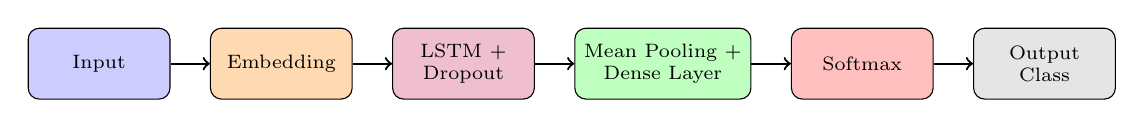
\begin{tikzpicture}[
                    node distance=0.8cm and 0.5cm,
                    every node/.style={align=center, font=\scriptsize},
                    layer/.style={draw, rounded corners, minimum height=0.9cm, minimum width=1.8cm, text centered},
                    input/.style={layer, fill=blue!20},
                    embed/.style={layer, fill=orange!30},
                    lstm/.style={layer, fill=purple!25},
                    dense/.style={layer, fill=green!25},
                    softmax/.style={layer, fill=red!25},
                    output/.style={layer, fill=gray!20}
                ]

                    % Nodes (horizontal layout)
                    \node (input) [input] {Input};
                    \node (embedding) [embed, right=of input] {Embedding};
                    \node (lstm) [lstm, right=of embedding] {LSTM + \\ Dropout};
                    \node (fc) [dense, right=of lstm] {Mean Pooling + \\ Dense Layer};
                    \node (sm) [softmax, right=of fc] {Softmax};
                    \node (out) [output, right=of sm] {Output \\ Class};

                    % Arrows
                    \draw[->, thick] (input) -- (embedding);
                    \draw[->, thick] (embedding) -- (lstm);
                    \draw[->, thick] (lstm) -- (fc);
                    \draw[->, thick] (fc) -- (sm);
                    \draw[->, thick] (sm) -- (out);

                \end{tikzpicture}
                \caption{LSTM-based sentiment classifier.}
            \end{figure}

            In particular, to evaluate the performance of the model, only the
            higher probability class is selected.
            The model is trained using the ADAM optimizer \citep{kingma2017adam},
            based on the cross-entropy loss function. Some form of dropout
            is applied to the LSTM layer to avoid overfitting.
            the model is trained for a maximum of 100 epochs, with early stopping
            kicking in almost always before the epochs upper limit, based on the 
            f1 score on the validation set.\\

            The tokenizer used in this model, as said before, is the NLTK tokenizer,
            with a vocabulary size of 10002, corresponding to the 10000 most
            frequent words in the training set, plus the \texttt{<PAD>} and \texttt{<OOV>} tokens,
            corresponding to the padding token and the out-of-vocabulary token.


        \subsubsection{RoBERTa Transformer}
        \label{subsubsec:roberta}
            The second model implemented is a \texttt{RoBERTaForSequenceClassification} transformer
            from the HuggingFace Transformers library, initialized at the \textit{roberta-base} 
            checkpoint. Furthermore, a classification MLP head is present, that takes information 
            from the first output of the RoBERTa transformer, which corresponds to the 
            \texttt{[CLS]} token, and maps it to the final output classes using softmax activation.

            \begin{figure}[H]
                \centering
                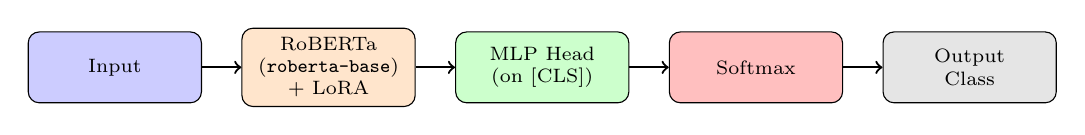
\begin{tikzpicture}[
                    node distance=0.8cm and 0.5cm,
                    every node/.style={align=center, font=\scriptsize},
                    layer/.style={draw, rounded corners, minimum height=0.9cm, minimum width=2.2cm, text centered},
                    input/.style={layer, fill=blue!20},
                    roberta/.style={layer, fill=orange!20},
                    mlp/.style={layer, fill=green!20},
                    softmax/.style={layer, fill=red!25},
                    output/.style={layer, fill=gray!20}
                ]

                    % Nodes (horizontal layout)
                    \node (input) [input] {Input};
                    \node (encoder) [roberta, right=of input] {RoBERTa\\(\texttt{roberta-base}) \\ + LoRA};
                    \node (mlp) [mlp, right=of encoder] {MLP Head\\(on [CLS])};
                    \node (sm) [softmax, right=of mlp] {Softmax};
                    \node (out) [output, right=of sm] {Output \\ Class};

                    % Arrows
                    \draw[->, thick] (input) -- (encoder);
                    \draw[->, thick] (encoder) -- (mlp);
                    \draw[->, thick] (mlp) -- (sm);
                    \draw[->, thick] (sm) -- (out);

                \end{tikzpicture}
                \caption{RoBERTa-based sentiment classifier.}
            \end{figure}

            The model, even though is pretrained, is fine-tuned on the datset using a rank-32 LoRA (Low-Rank Adaptation) PEFT
            with dropout. Like with the LSTM-RNN model the training has place using the cross-entropy loss function, 
            with the optimization performed using the ADAMW optimizer \citep{loshchilov2019decoupledweightdecayregularization}
            It should be noted that the model is trained using fp16 mixed precision, allowing
            to speed up the training and reducing the memory usage, allowing the
            training of the model on a single GPU with 6GB of memory.\\

            Furthermore, a Learning Rate Warmup \citep{kalra2024warmuplearningrateunderlying} of 10\% of the training steps
            is applied.
            The tokenizer used in this model is the \textit{roberta-base} tokenizer.
\section{Experimental analysis}
\label{sec:experimental_analysis}
    \subsection{Task}
      \label{sec:task}
        As mentioned in the introduction, the task consists in classifying sentences
        based on the sentiment expressed by them. after the training of the models,
        the desired output is a class, in the range from 1 to 5 stars in the first place,
        and in the range [0, 2] in the second place, where 0 is negative, 1 is neutral and
        2 is positive. \\
        
        Furthermore, such task is performed with the purpoose of not only gather 
        metrics about the generalization capabilities of the architectures implemented,
        but also to compare the performance of the two.
      

    \subsection{Experimental settings}
    Describe all the relevant aspects of the experimental setup used in your 
    experiment (e.g., how you performed model selection for fine-tuning of 
    hyper-parameters, all details regarding the learning / fine-tuning of your 
    model, etc.)
    \subsection{Results} 
    Provide results (figures and tables with mounerical results should go here). 
    Provide insights and comments on the achieved results (also comparatively with literature). Possible ablation studies go here.
\section{Discussion}
\label{sec:discussion}
    The results obtained from the experiments conducted on the Trip Advisor 
    reviews dataset provide valuable insights into the performance of
    current state-of-the-art models for sentiment analysis. 
    The comparison between the LSTM-RNN based models and the transformers
    based ones, particularly RoBERTa, highlights how different architectures
    can yield varying results depending on the nature of the dataset and the
    specific applications. \\

    LSTM models, despite requiring more epochs to converge, demostrated
    quite impactul results, achieving levels of performance in understanding 
    the sentiment expressed in the reviews that can be compared to Transformers
    architectures. On the other hand, Transformers, demonstrated that can be quite elastic
    in learning knowledge from very unbalanced datasets, particularly important
    in case of big datasets where oversampling techniques are unfeasible. \\

    In all the experiments, the hardest class to identify is the neutral one, 
    corresponding to the 3-star reviews. This limitation is likely due to the 
    inherent ambiguity in the language used in these reviews, which often
    includes mixed terminology and sentiments. Both models seem to struggle to "grasp 
    indecision" in the language, leading to lower accuracy and F1 scores.

    \subsection{Limitations}
    \label{sec:limitations}
        The main limitation about the choice of which model to use resides in the
        computational resources available, particularly at training time.
        Being trained on a consumer-grade GPU, Transformers models require 
        much more time to train, limited by the memory available on the GPU, besides
        the bigger amount of trainable parameters. Due to these limitations, it 
        was not possible to try larger models, such as larger versions of RoBERTa,
        that could have potentially yielded better results \\

        Another limitation is the size of the dataset, which is relatively small
        with respect to the complexity of the models used. It is easy to lead a model
        to overfitting, especially in the case of Transformers, which are known to
        require large amount of data to generalize well. Furthermore, the specificity
        of the dataset might lead to non generalizable results, thus limiting the 
        expected performance in other topics. \\
\section{Conclusions}
Draw conclusions and possibly delineate future works / possible improvements.

\bibliography{bib.bib}

\small

%%%%%%%%%%%%%%%%%%%%%%%%%%%%%%%%%%%%%%%%%%%%%%%%%%%%%%%%%%%%

\end{document}